\section{Results}
\label{sec:results}

\subsection{Why conventional evaluation is misleading}
\label{sec:res-split}
Under a conventional temporal split---train on the earliest 60\% of delegations, test on the latest 20\%---every method, including the blocklist, reaches an AUROC between $0.9998$ and $1.000$ with recall $1.0$ at a 1\% false-positive rate. The reason is that test delegations overwhelmingly target contracts, or exact clones of contracts, already seen in training. A family-disjoint split shows the same effect in miniature: on in-distribution families all methods reach $1.000$, whereas on held-out families the blocklist drops to $0.500$. Results on standard splits therefore measure memorisation of known contracts. Everything that follows uses the zero-day protocol, in which no contract, clone or family seen in training is evaluated.

\subsection{Zero-day detection}
\label{sec:res-zeroday}
Table~\ref{tab:zeroday} reports detection on unseen families, pooled over three folds and averaged over three seeds; Fig.~\ref{fig:zeroday} visualises the per-slice comparison and Fig.~\ref{fig:rocpr} the full ROC and precision--recall curves.

\begin{table*}[t]
\centering
\caption{Zero-day detection on unseen code families (mean $\pm$ std over three seeds; each delegation scored once per seed by a model that never saw its family). Recall is measured at the threshold giving 1\% false positives on validation families. Best value per column in bold.}
\label{tab:zeroday}
\footnotesize
\setlength{\tabcolsep}{3.2pt}
\begin{tabular}{l ccc ccc ccc}
\toprule
& \multicolumn{3}{c}{All delegations ($n{=}14{,}521$ per seed)} & \multicolumn{3}{c}{First ten victims per contract} & \multicolumn{3}{c}{First victim per contract ($n{=}60$)} \\
\cmidrule(lr){2-4}\cmidrule(lr){5-7}\cmidrule(lr){8-10}
Method & AUROC & AUPRC & MCC & AUROC & AUPRC & MCC & AUROC & AUPRC & MCC \\
\midrule
Blocklist & $0.500{\pm}.000$ & $0.780{\pm}.000$ & $0.000$ & $0.500{\pm}.000$ & $0.822{\pm}.000$ & $0.000$ & $0.500{\pm}.000$ & $0.817{\pm}.000$ & $0.000$ \\
Fuzzy hash & $0.975{\pm}.028$ & $0.993{\pm}.008$ & $0.550{\pm}.130$ & $0.947{\pm}.026$ & $0.986{\pm}.008$ & $0.433{\pm}.137$ & $0.918{\pm}.041$ & $0.977{\pm}.015$ & $0.415{\pm}.110$ \\
XGBoost & $0.998{\pm}.002$ & $\mathbf{1.000}{\pm}.000$ & $0.914{\pm}.126$ & $0.965{\pm}.025$ & $0.990{\pm}.008$ & $0.747{\pm}.043$ & $0.899{\pm}.054$ & $0.971{\pm}.018$ & $0.550{\pm}.074$ \\
GraphSAGE & $\mathbf{0.999}{\pm}.000$ & $\mathbf{1.000}{\pm}.000$ & $\mathbf{0.924}{\pm}.113$ & $\mathbf{0.975}{\pm}.000$ & $\mathbf{0.993}{\pm}.001$ & $0.761{\pm}.142$ & $0.898{\pm}.042$ & $0.974{\pm}.007$ & $0.563{\pm}.237$ \\
TGAT & $\mathbf{0.999}{\pm}.000$ & $\mathbf{1.000}{\pm}.000$ & $0.923{\pm}.121$ & $\mathbf{0.975}{\pm}.012$ & $0.992{\pm}.005$ & $\mathbf{0.774}{\pm}.129$ & $0.918{\pm}.045$ & $0.974{\pm}.020$ & $\mathbf{0.710}{\pm}.148$ \\
\textbf{\dn{}} & $0.982{\pm}.026$ & $0.995{\pm}.007$ & $0.654{\pm}.229$ & $0.967{\pm}.006$ & $0.992{\pm}.001$ & $0.568{\pm}.137$ & $\mathbf{0.946}{\pm}.009$ & $\mathbf{0.987}{\pm}.002$ & $0.551{\pm}.125$ \\
\bottomrule
\end{tabular}
\end{table*}

\begin{figure}[t]
\centering
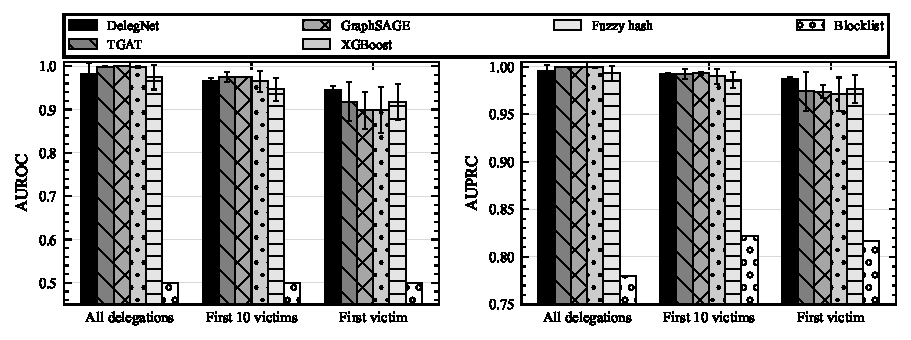
\includegraphics[width=0.4\textwidth]{fig_zeroday_slices}
\caption{Zero-day AUROC (left) and AUPRC (right) per evidence slice; bars show the mean over three seeds and whiskers one standard deviation. The blocklist is at chance on every slice. \dn{} has the highest mean on a contract's first victim and the smallest seed variance there.}
\label{fig:zeroday}
\end{figure}

\begin{figure}[t]
\centering
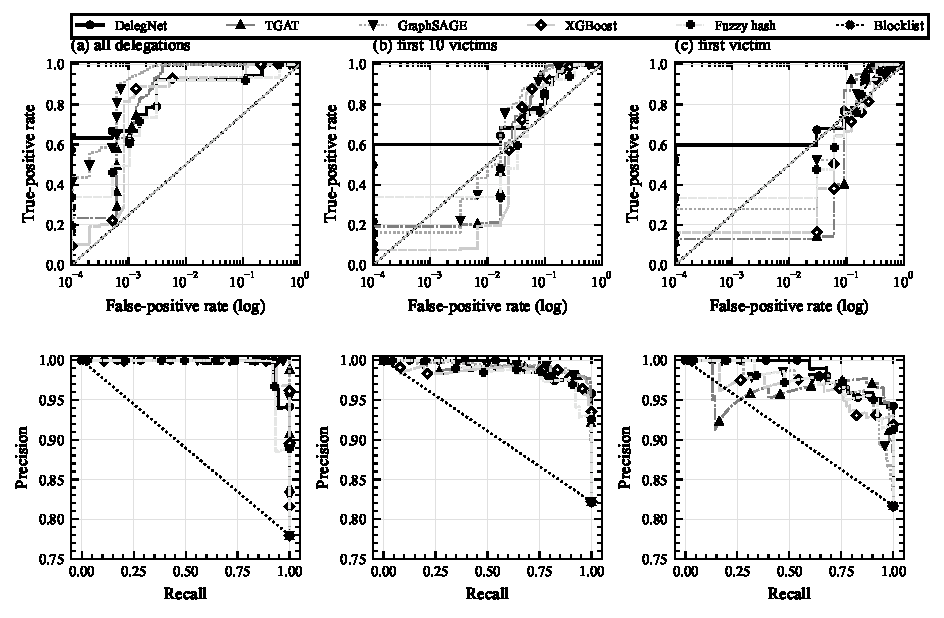
\includegraphics[width=0.4\textwidth]{fig_roc_pr}
\caption{ROC curves on a logarithmic false-positive axis (top) and precision--recall curves (bottom) for (a)~all delegations, (b)~the first ten victims and (c)~the first victim of each unseen contract, pooled over seeds.}
\label{fig:rocpr}
\end{figure}

Three findings stand out. First, the blocklist is at chance on every slice: an exact-match defence offers no protection against a new family, even when matching canonical rather than raw code. Second, on the full test population the temporal graph networks attain the highest AUROC ($0.999$) and \dn{} attains $0.982$. The graph models' advantage on this slice comes from sibling evidence: most test delegations belong to large campaigns whose earlier victims have already been drained by the time later victims delegate, which is visible to behavioural models but irrelevant to a code-based score. Third, on the \emph{first victim} of each new contract---where no sibling evidence exists and a detector must recognise the attack from what the contract is---\dn{} attains the highest AUROC ($0.946\pm0.009$), ahead of TGAT ($0.918$), fuzzy hashing ($0.918$), XGBoost ($0.899$) and GraphSAGE ($0.898$), with a seed standard deviation four to six times smaller than that of any learned baseline. Averaging three seeds raises \dn{}'s first-victim AUROC to $0.956$.

\paragraph{Score distributions} Fig.~\ref{fig:scores} shows why the code-based score generalises. On the first ten victims of unseen contracts, \dn{}'s malicious scores have interquartile range $[0.581, 0.662]$ and its benign scores $[0.413, 0.505]$; the ranges do not overlap, and the medians ($0.629$ and $0.459$) lie on either side of the indifference point $0.5$; the separation is produced by a contract's resemblance to theft code relative to wallet code, not by behaviour.

\begin{figure}[t]
\centering
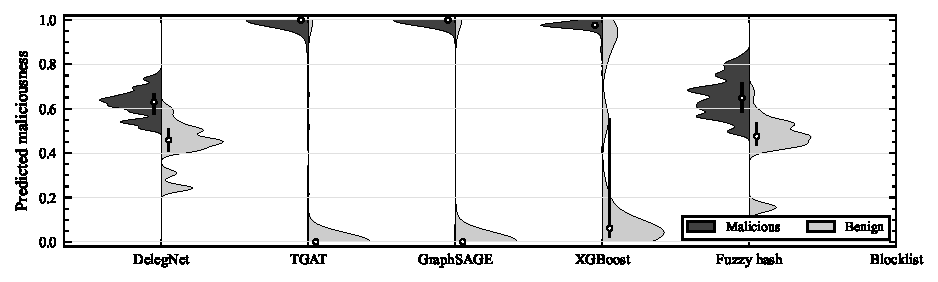
\includegraphics[width=0.4\textwidth]{fig_score_distributions}
\caption{Score distributions on the first ten victims of unseen contracts: malicious (dark, left half) and benign (light, right half) per method, with interquartile bars and medians.}
\label{fig:scores}
\end{figure}

\subsection{Effect of available evidence}
\label{sec:res-history}
Fig.~\ref{fig:history} resolves detection by the position of a delegation among its contract's victims. Behavioural models improve steeply as evidence accumulates: TGAT rises from $0.918$ on the first victim to $0.980$ for victims 2--10 and $1.000$ beyond the tenth, and GraphSAGE from $0.898$ to $1.000$. \dn{} is comparatively flat ($0.946$, $0.969$, $0.990$, $0.981$), because its decision does not depend on how many earlier victims have been drained. The two families of detectors are therefore strongest at opposite ends of a campaign. The first victims of a new campaign are, from a defender's perspective, the ones that matter most, since every later victim can in principle be protected by information about earlier ones; it is on these that \dn{} leads. The support panel of Fig.~\ref{fig:history} also explains why aggregate metrics favour behavioural models: per seed there are only $60$ first victims ($49$ malicious, $11$ benign), but $11{,}106$ delegations beyond the hundredth.

\begin{figure}[t]
\centering
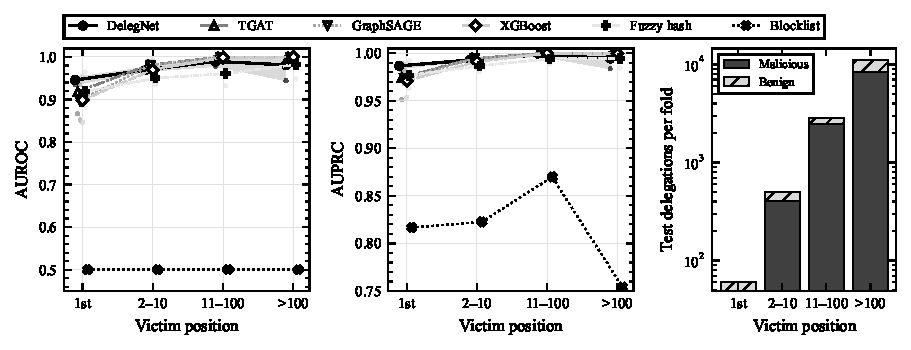
\includegraphics[width=0.4\textwidth]{fig_history_buckets}
\caption{Detection by evidence available at decision time. Left and centre: AUROC and AUPRC by the delegation's position among its contract's victims (mean line, per-seed points, \dn{}'s seed range shaded). Right: test support per bucket (malicious dark, benign hatched).}
\label{fig:history}
\end{figure}

\subsection{Robustness to code disguise}
\label{sec:res-disguise}
Fig.~\ref{fig:disguise} examines what happens when attackers re-deploy their contracts as semantics-preserving mutants. Panel~(b) shows the mechanism of failure for raw code matching: the four-gram similarity between a malicious contract and its mutant decays from $0.766$ at strength $0.25$ to $0.678$, $0.551$, $0.367$, $0.252$ and $0.192$ at strengths $0.5$ to $4$, uniformly across all $60$ contracts. Panel~(c) shows that the canonical form removes it: mean similarity stays at $0.999$--$1.000$ at every strength, and panel~(d) shows that this holds for each contract individually, with every point on the upper boundary regardless of its raw similarity.

The consequence for detection is shown in panel~(a). At the fixed operating threshold, fuzzy hashing's recall falls from $0.981$ to $0.822$ ($\sigma{=}0.5$), $0.579$ ($\sigma{=}1$) and $0.333$ ($\sigma{\ge}2$), whereas \dn{} remains at $0.984$ at every strength. Fuzzy hashing's AUROC is largely preserved ($0.991$), because mutation lowers malicious and benign similarities alike, but its scores collapse towards the indifference point, below any threshold set on clean data. A deployed fuzzy-hash detector would silently stop alerting. Detectors that do not read bytecode---the graph networks and the behavioural features of XGBoost---are unaffected by disguise, but, as the next experiment shows, are exposed to behavioural manipulation instead.

\begin{figure}[t]
\centering
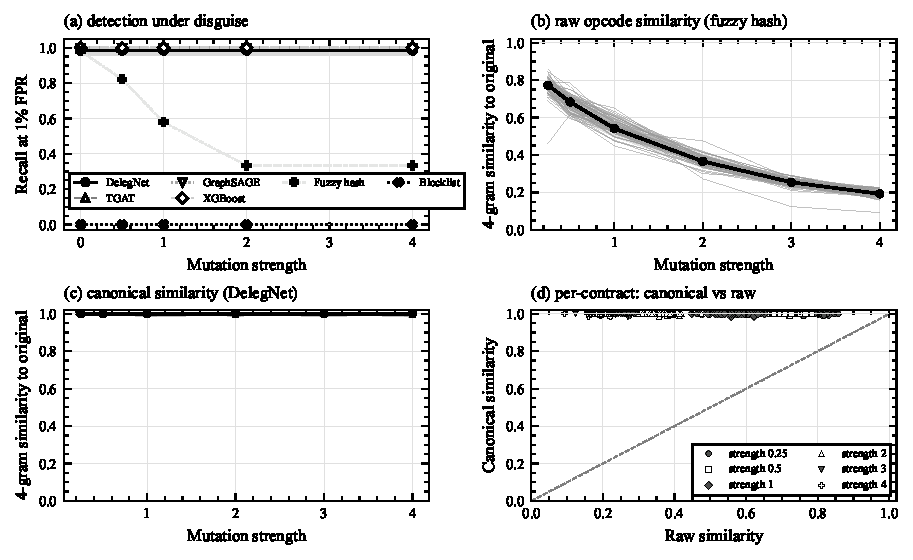
\includegraphics[width=0.4\textwidth]{fig_code_disguise}
\caption{Code disguise. (a)~Recall at 1\% FPR as mutation strength grows. (b)~Raw opcode four-gram similarity between each of 60 malicious contracts and its mutant (thin lines), with median, interquartile and 10--90\% bands. (c)~The same for \dn{}'s canonical form. (d)~Per-contract canonical versus raw similarity at six strengths.}
\label{fig:disguise}
\end{figure}

\subsection{Robustness to adaptive attackers}
\label{sec:res-evasion}
Table~\ref{tab:evasion} and Figs.~\ref{fig:evasion}--\ref{fig:evasion-prof} report the five-attack suite.

\begin{table}[t]
\centering
\caption{Recall at the clean-data 1\% FPR threshold under adaptive attacks (mean over three seeds; last zero-day fold of each seed). Attacks modify only attacker-controlled inputs of malicious delegations.}
\label{tab:evasion}
\footnotesize
\setlength{\tabcolsep}{2.4pt}
\begin{tabular}{lcccccc}
\toprule
Method & None & Self-sub. & Fresh spons. & Fresh contr. & Disguise & Combined \\
\midrule
Blocklist & 0.000 & 0.000 & 0.000 & 0.000 & 0.000 & 0.000 \\
Fuzzy hash & 0.981 & 0.981 & 0.981 & 0.981 & 0.333 & 0.333 \\
XGBoost & 1.000 & 0.666 & 0.667 & 1.000 & 1.000 & 0.667 \\
GraphSAGE & 1.000 & 0.548 & 1.000 & 1.000 & 1.000 & 0.229 \\
TGAT & 1.000 & 0.450 & 0.967 & 1.000 & 1.000 & 0.228 \\
\textbf{\dn{}} & \textbf{0.984} & \textbf{0.984} & \textbf{0.984} & \textbf{0.984} & \textbf{0.984} & \textbf{0.984} \\
\bottomrule
\end{tabular}
\end{table}

\begin{figure}[t]
\centering
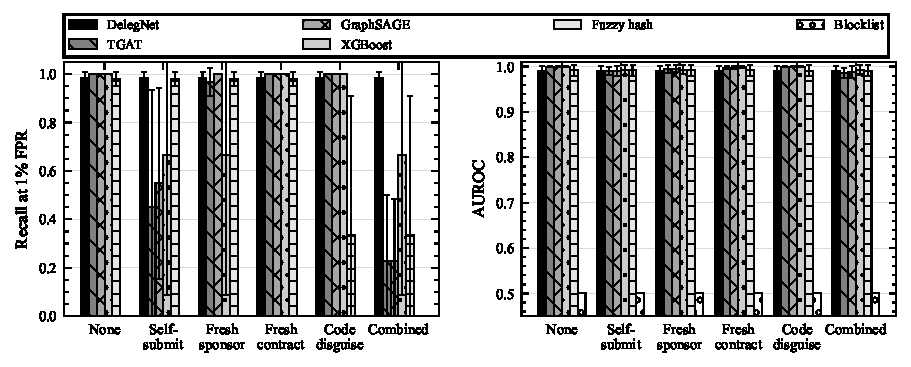
\includegraphics[width=0.4\textwidth]{fig_evasion_suite}
\caption{Adaptive-adversary suite: recall at the clean-data 1\% FPR threshold (left) and AUROC (right) for every method under each attack; whiskers show one standard deviation over seeds.}
\label{fig:evasion}
\end{figure}

\begin{figure}[t]
\centering
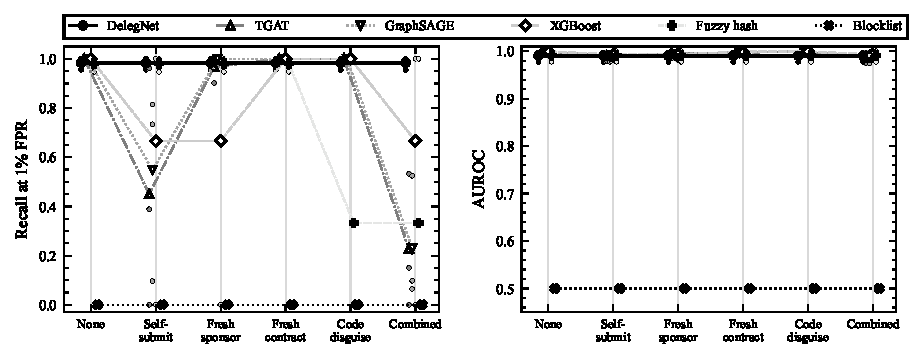
\includegraphics[width=0.4\textwidth]{fig_evasion_profiles}
\caption{Attack profiles: each line traces a method's mean recall (left) and AUROC (right) across attacks, with per-seed points. \dn{}'s profile is flat; behavioural detectors dip under self-submission and the combined attack.}
\label{fig:evasion-prof}
\end{figure}

\paragraph{Behavioural evasion} A single, costless change---submitting the authorization from the victim's own account instead of through a sponsor---reduces TGAT's recall from $1.000$ to $0.450$, GraphSAGE's to $0.548$ and XGBoost's to $0.666$. The models learned that sponsored, batched submission is characteristic of current campaigns. The feature is genuinely predictive on present data and entirely under the attacker's control. A fresh sponsor per victim primarily affects XGBoost ($0.667$), whose features include sponsor breadth and funding. The combined attack reduces both graph networks to $0.23$ recall: more than three quarters of malicious delegations pass undetected at the operating point. The graph networks' AUROC degrades only modestly ($0.986$--$0.990$), which shows that the attacks shift malicious scores downward across the board rather than scrambling their order. In deployment, however, a detector must commit to a threshold before it knows an attack is under way, and at that threshold the shift is decisive.

\paragraph{\dn{}} \dn{}'s recall is $0.984$ under every attack, identical to its clean-data recall, with AUROC $0.991$ throughout. This invariance follows from the design rather than from tuning: the score depends only on the delegate's canonical code, the behavioural attacks change nothing that it reads, and the disguise attack changes nothing that survives canonicalisation. The only way to evade \dn{} is to change what the contract does, and doing so means writing a new theft mechanism rather than re-using one.

\subsection{Screening before signing}
\label{sec:res-presig}
Because two thirds of thefts complete in the authorization's own block, protection must occur when the wallet asks the user to sign. Table~\ref{tab:presig} and Fig.~\ref{fig:presig} evaluate every method at that moment, when the signer and delegate are known but the sponsor is not.

\begin{table}[t]
\centering
\caption{Pre-signature screening (mean $\pm$ std over seeds): AUROC, recall and benign false-alarm rate at the clean-data operating threshold.}
\label{tab:presig}
\footnotesize
\setlength{\tabcolsep}{3.5pt}
\begin{tabular}{lccc}
\toprule
Method & AUROC & Recall & False alarms \\
\midrule
Blocklist & $0.500{\pm}.000$ & $0.000{\pm}.000$ & $0.000{\pm}.000$ \\
Fuzzy hash & $0.992{\pm}.012$ & $0.981{\pm}.029$ & $\mathbf{0.002}{\pm}.003$ \\
XGBoost & $\mathbf{0.999}{\pm}.001$ & $0.666{\pm}.576$ & $0.003{\pm}.005$ \\
GraphSAGE & $0.959{\pm}.043$ & $0.535{\pm}.329$ & $0.034{\pm}.030$ \\
TGAT & $0.931{\pm}.109$ & $0.501{\pm}.497$ & $0.189{\pm}.185$ \\
\textbf{\dn{}} & $0.991{\pm}.011$ & $\mathbf{0.984}{\pm}.025$ & $\mathbf{0.002}{\pm}.003$ \\
\bottomrule
\end{tabular}
\end{table}

\begin{figure}[t]
\centering
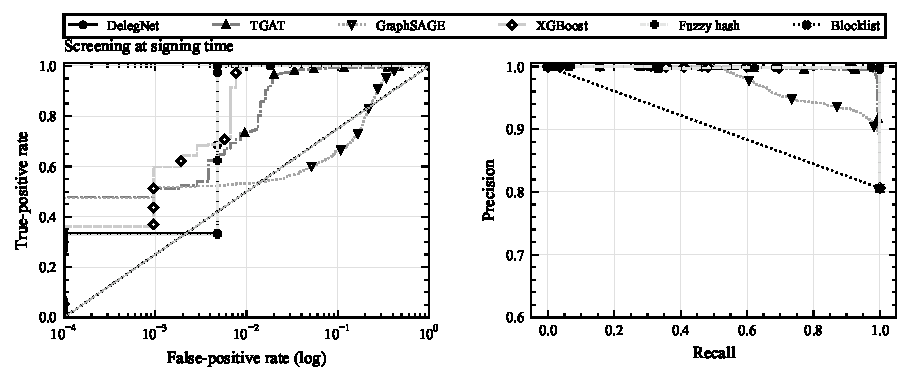
\includegraphics[width=0.4\textwidth]{fig_presignature}
\caption{Screening at signing time: ROC curves on a logarithmic false-positive axis (left) and precision--recall curves (right), seed~0, last zero-day fold.}
\label{fig:presig}
\end{figure}

\dn{} detects $98.4\%$ of malicious delegation requests with a false-alarm rate of $0.16\%$---roughly one unnecessary warning per $600$ benign delegations---and is stable across seeds. The behavioural detectors lose the evidence they rely on: without the sponsor and the authorization event, TGAT's recall falls to $0.501$ with an $18.9\%$ false-alarm rate, and GraphSAGE's to $0.535$ at $3.4\%$. XGBoost ranks pre-signature requests well (AUROC $0.999$, since it also reads code idioms), but its recall at the operating threshold varies between seeds from $0$ to $1$ ($0.666\pm0.576$). Its threshold, calibrated on post-inclusion behaviour, does not transfer to the pre-signature distribution of its inputs. Fuzzy hashing matches \dn{} at signing time on clean code, but it inherits the $0.333$ recall of Section~\ref{sec:res-disguise} as soon as attackers mutate their bytecode.

\subsection{Post-inclusion monitoring}
\label{sec:res-monitor}
Table~\ref{tab:monitor} evaluates a monitoring deployment that scores delegations at checkpoints after inclusion and blocks further outflows on alert.

\begin{table}[t]
\centering
\caption{Post-inclusion monitoring (last zero-day fold, mean over seeds): share of malicious delegations alerted, share alerted before their first theft, share of stolen value leaving after the alert, benign false-alarm rate, and AUROC at inclusion and two hours later.}
\label{tab:monitor}
\footnotesize
\setlength{\tabcolsep}{2.2pt}
\begin{tabular}{lcccccc}
\toprule
Method & Alerted & Pre-theft & Value saved & False al. & AUC@0s & AUC@2h \\
\midrule
Blocklist & 0.000 & 0.000 & 0.000 & 0.000 & 0.500 & 0.500 \\
Fuzzy hash & 0.981 & 0.994 & 0.999 & 0.002 & 0.992 & 0.992 \\
XGBoost & 1.000 & 1.000 & 1.000 & 0.007 & 1.000 & 1.000 \\
GraphSAGE & 1.000 & 1.000 & 1.000 & 0.011 & 1.000 & 1.000 \\
TGAT & 1.000 & 1.000 & 1.000 & 0.023 & 1.000 & 1.000 \\
\textbf{\dn{}} & 0.984 & 0.995 & 0.999 & \textbf{0.002} & 0.991 & 0.991 \\
\bottomrule
\end{tabular}
\end{table}

All learned detectors alert on nearly every malicious delegation at the moment of inclusion and before its first theft is recorded. \dn{} does so with the lowest false-alarm rate ($0.16\%$, against $0.7$--$2.3\%$ for the behavioural models), which matters at the scale of $634{,}828$ delegations in two months. The pre-theft figure must, however, be read alongside the dataset statistics: $67.7\%$ of thefts occur within the authorization's own block, typically in the very transaction that carries it, so an alert raised after inclusion cannot stop them. Monitoring is therefore a complement to, not a substitute for, screening before signing, where \dn{} is the only reliable method.

\subsection{Contract-level reliability and statistical significance}
\label{sec:res-contract}
Fig.~\ref{fig:contract} examines the $60$ held-out contracts individually. The heatmap shows each contract's mean score over its first ten victims, and the violins show bootstrap distributions of contract-level AUROC. \dn{} separates malicious from benign contracts with AUROC $0.952$ [0.869, 1.000], compared with $0.987$ [0.956, 1.000] for TGAT, $0.983$ for GraphSAGE, $0.964$ for fuzzy hashing and $0.891$ [0.740, 1.000] for XGBoost. Table~\ref{tab:sig} reports paired bootstrap comparisons on identical delegations. On the first victim and the first ten victims, \dn{}'s differences to every learned baseline lie within bootstrap uncertainty, a consequence of having $60$ first victims per seed and only $11$ labelled benign contracts. On the full population the graph networks are significantly more accurate, by $0.017$ AUROC, reflecting their use of sibling evidence on later victims. Against the blocklist, \dn{} is better by $0.45$--$0.48$ AUROC on every slice ($p<0.001$). The decisive differences in favour of \dn{} are those of Sections~\ref{sec:res-disguise}--\ref{sec:res-presig}: a recall of $0.984$ against $0.228$--$0.333$ under attack, and against $0.50$--$0.54$ for graph networks before signing.

\begin{figure}[t]
\centering
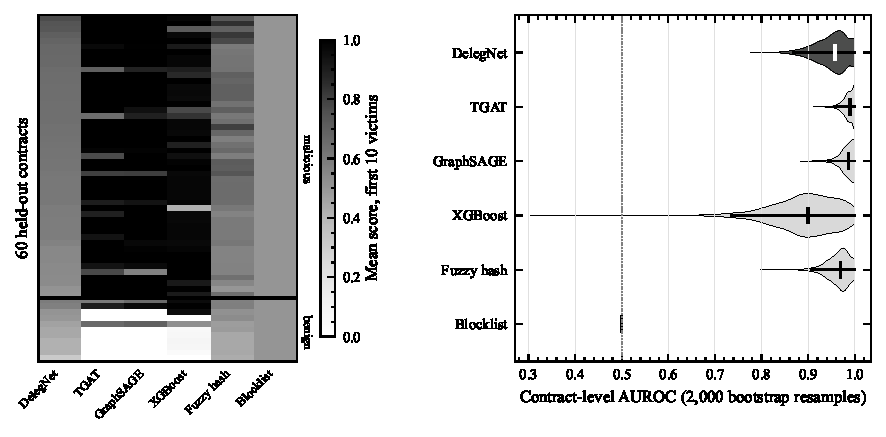
\includegraphics[width=0.4\textwidth]{fig_contract_level}
\caption{Contract-level analysis. Left: mean score over the first ten victims for every held-out contract (rows; malicious above the line, benign below) and method (columns). Right: contract-level AUROC over 2{,}000 bootstrap resamples of contracts, with 95\% intervals and medians.}
\label{fig:contract}
\end{figure}

\begin{table}[t]
\centering
\caption{Paired bootstrap difference in AUROC (\dn{} minus baseline), mean over seeds, with 95\% interval.}
\label{tab:sig}
\footnotesize
\setlength{\tabcolsep}{3pt}
\begin{tabular}{lccc}
\toprule
Baseline & All & First 10 & First victim \\
\midrule
Blocklist & $+0.482$ [0.481, 0.484] & $+0.467$ [0.448, 0.482] & $+0.446$ [0.360, 0.500] \\
Fuzzy hash & $+0.008$ [0.005, 0.010] & $+0.020$ [0.006, 0.034] & $+0.027$ [$-0.023$, 0.087] \\
XGBoost & $-0.016$ [$-0.018$, $-0.014$] & $+0.002$ [$-0.019$, 0.023] & $+0.045$ [$-0.039$, 0.143] \\
GraphSAGE & $-0.017$ [$-0.019$, $-0.016$] & $-0.008$ [$-0.024$, 0.009] & $+0.048$ [$-0.032$, 0.148] \\
TGAT & $-0.017$ [$-0.019$, $-0.015$] & $-0.008$ [$-0.027$, 0.012] & $+0.029$ [$-0.065$, 0.141] \\
\bottomrule
\end{tabular}
\end{table}

\subsection{Validity audit}
\label{sec:res-validity}
Fig.~\ref{fig:leak} reports the label-permutation and shuffled-label checks. For every learned method the observed test AUROC lies far outside the null distribution obtained by permuting test labels $1{,}000$ times (null mean $0.500$, 97.5th percentile $\le 0.558$, permutation $p=0.001$, the smallest attainable), so all reported separations are statistically real. When XGBoost is retrained on class-balanced data with shuffled labels, its test AUROC falls to $0.38\pm0.10$ on all delegations and $0.44\pm0.09$ on first victims: no path in the pipeline carries label information when the training labels carry none. Train, validation and test AUROC for the final fold are $1.000$, $1.000$ and $0.997$ for \dn{}, $1.000$, $1.000$ and $0.999$ for TGAT and GraphSAGE, and $1.000$, $1.000$ and $0.999$ for XGBoost; no method exhibits a train--test gap indicative of overfitting.

\begin{figure}[t]
\centering
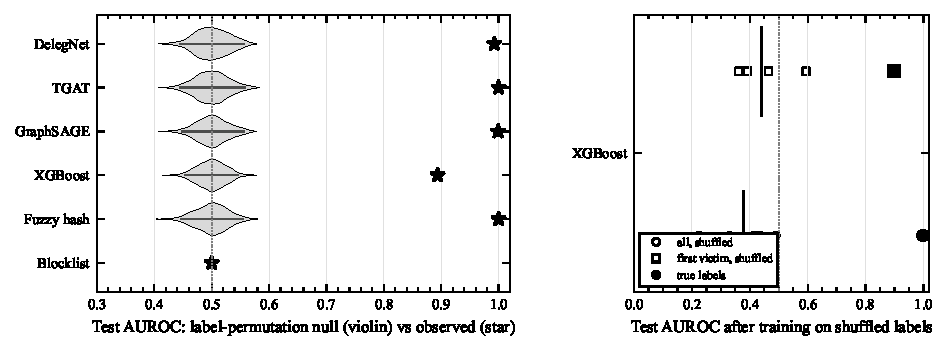
\includegraphics[width=0.4\textwidth]{fig_leakage_audit}
\caption{Validity audit. Left: null distributions of test AUROC under 1{,}000 permutations of test labels (violins, 95\% bars) versus observed AUROC (stars). Right: test AUROC after retraining on class-balanced shuffled labels (open markers; bars give the mean) versus training on true labels (filled).}
\label{fig:leak}
\end{figure}

\subsection{Summary of capabilities}
Fig.~\ref{fig:capability} condenses the evaluation. The behavioural graph networks are the most accurate detectors when attackers behave as they did in the observed campaigns and evidence about earlier victims is available. Every capability that depends on resisting an adaptive attacker or acting before signing, however, is held by \dn{} alone: first-victim detection ($0.946$), recall under the combined attack ($0.984$), under self-submission ($0.984$), under code disguise ($0.984$) and before signing ($0.984$).

\begin{figure}[t]
\centering
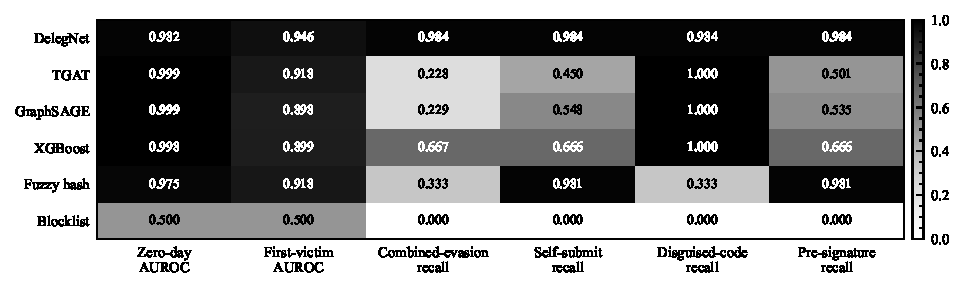
\includegraphics[width=0.4\textwidth]{fig_capability_matrix}
\caption{Capability matrix: zero-day AUROC, first-victim AUROC, and recall at 1\% FPR under the combined attack, self-submission, code disguise ($\sigma{=}4$) and before signing. Bold marks the best value per column.}
\label{fig:capability}
\end{figure}
